\chapter{Channel Models: Rayleigh and Rician Fading}
\label{ch:channel-models-rayleigh-rician}

\begin{nontechnical}
\textbf{Channel models are like flight simulators for radio engineers}---they let you test communication systems in virtual cities, tunnels, and open fields before building real hardware.

\textbf{The problem:}
\begin{itemize}
\item Can't test every scenario (urban, suburban, highway, indoor)
\item Real-world testing is expensive (hardware, locations, permits)
\item Need to test extreme conditions (rain, crowds, interference)
\item Can't test satellites or Mars missions easily!
\end{itemize}

\textbf{The solution---mathematical simulation:}
\begin{itemize}
\item Create computer models of radio environments
\item Run communication system in simulation
\item Measure performance before building hardware
\end{itemize}

\textbf{The two main models:}

\textbf{1. Rayleigh fading} (no line-of-sight):
\begin{itemize}
\item \textbf{Environment:} Dense urban, indoors, tunnels
\item \textbf{Characteristic:} Signal bounces everywhere, no direct path
\item \textbf{Result:} Wild signal fluctuations (30+ dB swings!)
\item \textbf{Example:} Walking through downtown, WiFi in building with walls
\end{itemize}

\textbf{2. Rician fading} (strong line-of-sight + scatter):
\begin{itemize}
\item \textbf{Environment:} Suburban, rural, highways, open areas
\item \textbf{Characteristic:} One strong direct path + weaker echoes
\item \textbf{Result:} More stable signal, less severe fading
\item \textbf{Example:} Highway cell tower, rural WiFi
\end{itemize}

\textbf{Why simulation matters:} When engineers designed the LTE standard (4G), they ran over 1 million simulations using standardized channel models. This is why 4G ``just worked'' globally from day one---they'd already tested every conceivable environment virtually.
\end{nontechnical}

\section{Overview}

\textbf{Channel models} mathematically simulate wireless propagation effects, enabling system design and performance prediction without hardware deployment.

\begin{keyconcept}
Channel models bridge theory and practice: they capture real-world multipath, fading, and Doppler effects in computational form, allowing engineers to test millions of scenarios before committing to hardware.
\end{keyconcept}

\textbf{Primary applications:}
\begin{itemize}
\item \textbf{System simulation:} Test modulation/coding schemes under realistic conditions
\item \textbf{Performance prediction:} Estimate BER vs SNR for different environments
\item \textbf{Algorithm development:} Design equalizers and synchronizers
\item \textbf{Standards compliance:} 3GPP and ITU specify reference channel models
\end{itemize}

\textbf{Model hierarchy:}
\begin{enumerate}
\item \textbf{AWGN:} Ideal baseline (additive white Gaussian noise only)
\item \textbf{Flat fading:} Narrowband channels with single complex gain
\item \textbf{Frequency-selective fading:} Wideband channels with delay spread (ISI)
\end{enumerate}

\section{Mathematical Description}

\subsection{AWGN Channel (Baseline)}

The simplest channel model adds only white Gaussian noise to the transmitted signal:
\begin{equation}
r(t) = s(t) + n(t)
\end{equation}
where:
\begin{itemize}
\item $r(t)$ = received signal
\item $s(t)$ = transmitted signal
\item $n(t)$ = additive white Gaussian noise with variance $\sigma^2 = N_0 B$
\end{itemize}

The noise power spectral density $N_0$ and bandwidth $B$ determine the total noise power:
\begin{equation}
P_n = N_0 \cdot B
\end{equation}

\subsection{Flat Fading Channel Model}

For narrowband systems where signal bandwidth $B \ll B_c$ (coherence bandwidth), the channel introduces a single complex gain:
\begin{equation}
r(t) = h(t) \cdot s(t) + n(t)
\end{equation}
where:
\begin{itemize}
\item $h(t)$ = complex channel gain (time-varying)
\item $|h(t)|$ = amplitude (Rayleigh or Rician distributed)
\item $\angle h(t)$ = phase (uniformly distributed)
\end{itemize}

The flat fading approximation is valid when:
\begin{equation}
T_s \gg \tau_{\text{rms}}
\end{equation}
where $T_s$ is symbol duration and $\tau_{\text{rms}}$ is RMS delay spread.

\subsection{Rayleigh Fading Model}

\subsubsection{Physical Basis}

Rayleigh fading occurs in non-line-of-sight (NLOS) environments where many scattered paths arrive with equal power. The central limit theorem dictates that the received signal is a complex Gaussian random variable.

\textbf{Statistical properties:}

The envelope $r = |h(t)|$ follows the \textbf{Rayleigh distribution}:
\begin{equation}
p(r) = \frac{r}{\sigma^2} \exp\left(-\frac{r^2}{2\sigma^2}\right), \quad r \geq 0
\end{equation}
where:
\begin{itemize}
\item $\sigma^2$ = average power per dimension (I and Q)
\item For normalized power: $\sigma^2 = 1/2$ so that $E[|h|^2] = 1$
\end{itemize}

\textbf{Mean and variance:}
\begin{equation}
E[r] = \sigma\sqrt{\frac{\pi}{2}}, \quad \mathrm{Var}(r) = \sigma^2\left(2 - \frac{\pi}{2}\right)
\end{equation}

\subsubsection{Clarke's Doppler Spectrum}

For isotropic scattering (scatterers uniformly distributed in azimuth), the Doppler spectrum has a characteristic U-shape:
\begin{equation}
S(f) = \frac{1}{\pi f_d \sqrt{1 - (f/f_d)^2}}, \quad |f| < f_d
\end{equation}
where:
\begin{itemize}
\item $f_d = v/\lambda$ = maximum Doppler frequency (Hz)
\item $v$ = mobile velocity (m/s)
\item $\lambda$ = wavelength (m)
\end{itemize}

The autocorrelation function is:
\begin{equation}
R(\tau) = J_0(2\pi f_d \tau)
\end{equation}
where $J_0$ is the Bessel function of the first kind, order 0.

\subsubsection{Jakes' Model Implementation}

Jakes' model efficiently generates Rayleigh fading using a sum of sinusoids:

\textbf{In-phase component:}
\begin{equation}
h_I(t) = \frac{1}{\sqrt{M}} \sum_{m=1}^{M} \cos(2\pi f_d t \cos\theta_m + \phi_m)
\end{equation}

\textbf{Quadrature component:}
\begin{equation}
h_Q(t) = \frac{1}{\sqrt{M}} \sum_{m=1}^{M} \sin(2\pi f_d t \cos\theta_m + \phi_m)
\end{equation}
where:
\begin{itemize}
\item $M$ = number of scatterers (typically 8--16)
\item $\theta_m = \frac{2\pi m}{M}$ = equally spaced angles
\item $\phi_m$ = random phases, uniform on $[0, 2\pi]$
\end{itemize}

The complex channel gain is:
\begin{equation}
h(t) = \frac{1}{\sqrt{2}}\left[h_I(t) + jh_Q(t)\right]
\end{equation}

The $1/\sqrt{2}$ normalization ensures $E[|h(t)|^2] = 1$.

\subsection{Rician Fading Model}

\subsubsection{Physical Basis}

Rician fading occurs when a dominant line-of-sight (LOS) path exists alongside scattered multipath components. This is typical in suburban, rural, and highway environments.

\textbf{Statistical properties:}

The envelope follows the \textbf{Rician distribution}:
\begin{equation}
p(r) = \frac{r}{\sigma^2} \exp\left(-\frac{r^2 + A^2}{2\sigma^2}\right) I_0\left(\frac{Ar}{\sigma^2}\right)
\end{equation}
where:
\begin{itemize}
\item $A$ = amplitude of LOS component
\item $\sigma^2$ = power per dimension of scattered component
\item $I_0(\cdot)$ = modified Bessel function of the first kind, order 0
\end{itemize}

\subsubsection{K-Factor}

The \textbf{K-factor} quantifies the ratio of LOS power to scattered power:
\begin{equation}
K = \frac{A^2}{2\sigma^2} = \frac{P_{\text{LOS}}}{P_{\text{scatter}}}
\end{equation}

In decibels:
\begin{equation}
K_{\text{dB}} = 10\log_{10}(K)
\end{equation}

\textbf{Special cases:}
\begin{itemize}
\item $K = 0$ ($K = -\infty$~dB): Pure Rayleigh fading (no LOS)
\item $K = 10$ ($K = 10$~dB): Strong LOS (typical suburban)
\item $K \to \infty$: Pure LOS (AWGN-like channel)
\end{itemize}

\textbf{Normalized Rician channel:}

For unit average power $E[|h|^2] = 1$:
\begin{equation}
h_{\text{LOS}} = \sqrt{\frac{K}{K+1}}, \quad \sigma^2_{\text{scatter}} = \frac{1}{2(K+1)}
\end{equation}

The channel gain becomes:
\begin{equation}
h(t) = \sqrt{\frac{K}{K+1}} + \sqrt{\frac{1}{K+1}} \cdot h_{\text{Rayleigh}}(t)
\end{equation}

\subsection{Visual Comparison: Rayleigh vs Rician Distributions}

\begin{center}
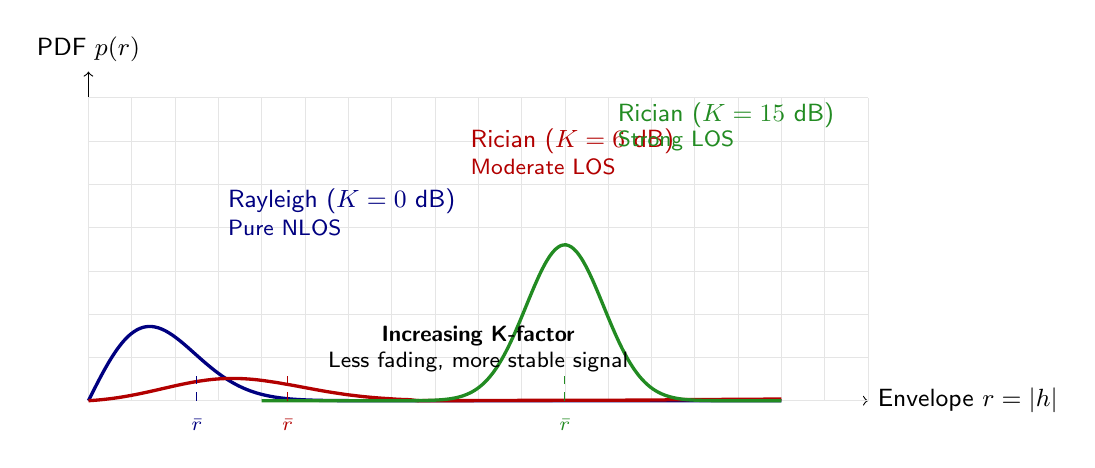
\begin{tikzpicture}[scale=1.1]
% Axes
\draw[->] (0,0) -- (9,0) node[right,font=\sffamily\small] {Envelope $r = |h|$};
\draw[->] (0,0) -- (0,3.8) node[above,font=\sffamily\small] {PDF $p(r)$};

% Grid
\draw[very thin,gray!20] (0,0) grid[step=0.5] (9,3.5);

% Rayleigh PDF (K=0, pure NLOS)
\draw[NavyBlue, very thick, smooth, domain=0:8, samples=100] 
  plot (\x, {2*\x*exp(-\x*\x)});
\node[NavyBlue,font=\sffamily\small,anchor=west] at (1.5,2.3) {Rayleigh ($K=0$ dB)};
\node[NavyBlue,font=\sffamily\footnotesize,anchor=west] at (1.5,2.0) {Pure NLOS};

% Rician PDF K=6 dB (K=4 linear)
\draw[red!70!black, very thick, smooth, domain=0:8, samples=100] 
  plot (\x, {0.45*\x*exp(-(\x*\x + 4)/2)*
    (1 + 4*(\x/2) + 8*(\x/2)*(\x/2)/2 + 32*(\x/2)*(\x/2)*(\x/2)/6)});
\node[red!70!black,font=\sffamily\small,anchor=west] at (4.3,3.0) {Rician ($K=6$ dB)};
\node[red!70!black,font=\sffamily\footnotesize,anchor=west] at (4.3,2.7) {Moderate LOS};

% Rician PDF K=15 dB (K=31.6 linear)
\draw[ForestGreen, very thick, smooth, domain=2:8, samples=100] 
  plot (\x, {1.8*exp(-(\x-5.5)*(\x-5.5)/0.4)});
\node[ForestGreen,font=\sffamily\small,anchor=west] at (6.0,3.3) {Rician ($K=15$ dB)};
\node[ForestGreen,font=\sffamily\footnotesize,anchor=west] at (6.0,3.0) {Strong LOS};

% Mean markers
\draw[NavyBlue,dashed] (1.25,0) -- (1.25,0.3);
\node[NavyBlue,below,font=\scriptsize] at (1.25,-0.1) {$\bar{r}$};

\draw[red!70!black,dashed] (2.3,0) -- (2.3,0.3);
\node[red!70!black,below,font=\scriptsize] at (2.3,-0.1) {$\bar{r}$};

\draw[ForestGreen,dashed] (5.5,0) -- (5.5,0.3);
\node[ForestGreen,below,font=\scriptsize] at (5.5,-0.1) {$\bar{r}$};

% Annotations
\node[font=\sffamily\footnotesize,align=center] at (4.5,0.6) {
  \textbf{Increasing K-factor} \\
  Less fading, more stable signal
};

\end{tikzpicture}
\end{center}

\begin{calloutbox}{Physical Interpretation}
\begin{itemize}
\item \textbf{Rayleigh (blue):} Broad distribution, high probability of deep fades near $r=0$
\item \textbf{Rician K=6~dB (red):} Narrower, reduced deep fade probability
\item \textbf{Rician K=15~dB (green):} Concentrated around mean, approaches constant channel
\end{itemize}
As $K$ increases, the channel transitions from severe fading (Rayleigh) to nearly constant (AWGN).
\end{calloutbox}

\subsection{Block Diagram: Fading Channel Simulator}

\begin{center}
\begin{tikzpicture}[
  block/.style={rectangle, draw, minimum width=2.2cm, minimum height=1cm, font=\sffamily\small, align=center},
  node distance=2cm,
  font=\small
]
\node (input) {\sffamily Baseband\\Signal\\$s(t)$};
\node[block, right of=input] (fading) {Rayleigh/Rician\\Fading\\Generator};
\node[block, right of=fading] (multiply) {Complex\\Multiply};
\node[block, right of=multiply] (awgn) {AWGN};
\node[right of=awgn] (output) {\sffamily Received\\Signal\\$r(t)$};

% Signal flow
\draw[->,thick] (input) -- (multiply);
\draw[->,thick] (fading) -- node[above,font=\scriptsize] {$h(t)$} (multiply);
\draw[->,thick] (multiply) -- node[above,font=\scriptsize] {$h(t) \cdot s(t)$} (awgn);
\draw[->,thick] (awgn) -- (output);

% Parameters
\node[block, below=1.5cm of fading, minimum width=2.5cm] (params) {Parameters:\\$f_d$, $K$-factor\\(Doppler, LOS)};
\draw[->,thick] (params) -- (fading);

% Noise source
\node[block, below=1.5cm of awgn, minimum width=1.8cm] (noise) {Noise\\Generator\\$n(t)$};
\draw[->,thick] (noise) -- (awgn);

\end{tikzpicture}
\end{center}

\section{Channel Impulse Response}

\subsection{Time-Varying Channel Visualization}

\begin{center}
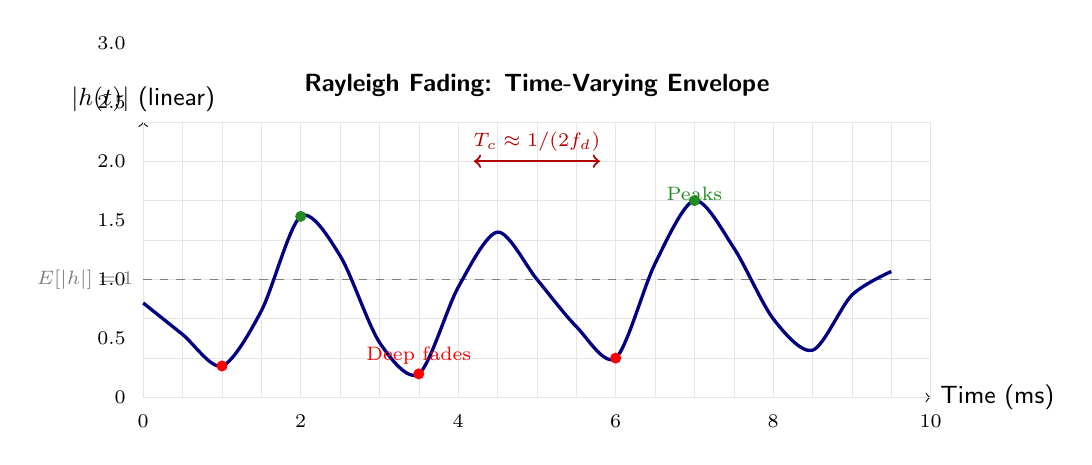
\begin{tikzpicture}[scale=1.0]
% Time axis (horizontal)
\draw[->] (0,0) -- (10,0) node[right,font=\sffamily\small] {Time (ms)};

% Amplitude axis (vertical)
\draw[->] (0,0) -- (0,3.5) node[above,font=\sffamily\small] {$|h(t)|$ (linear)};

% Grid
\draw[very thin,gray!20] (0,0) grid[step=0.5] (10,3.5);

% Reference line at |h|=1 (average power)
\draw[dashed,gray] (0,1.5) -- (10,1.5);
\node[gray,font=\scriptsize,left] at (0,1.5) {$E[|h|]=1$};

% Rayleigh fading envelope (simulated with random-looking curve)
\draw[NavyBlue, very thick, smooth] 
  plot coordinates {
    (0,1.2) (0.5,0.8) (1.0,0.4) (1.5,1.1) (2.0,2.3) 
    (2.5,1.8) (3.0,0.7) (3.5,0.3) (4.0,1.4) (4.5,2.1)
    (5.0,1.5) (5.5,0.9) (6.0,0.5) (6.5,1.7) (7.0,2.5)
    (7.5,1.9) (8.0,1.0) (8.5,0.6) (9.0,1.3) (9.5,1.6)
  };

% Deep fade markers
\fill[red] (1.0,0.4) circle (2pt);
\fill[red] (3.5,0.3) circle (2pt);
\fill[red] (6.0,0.5) circle (2pt);
\node[red,font=\scriptsize,above] at (3.5,0.3) {Deep fades};

% Peak markers
\fill[ForestGreen] (2.0,2.3) circle (2pt);
\fill[ForestGreen] (7.0,2.5) circle (2pt);
\node[ForestGreen,font=\scriptsize,below] at (7.0,2.8) {Peaks};

% Coherence time annotation
\draw[<->,thick,red!70!black] (4.2,3.0) -- (5.8,3.0);
\node[red!70!black,font=\scriptsize,above] at (5.0,3.0) {$T_c \approx 1/(2f_d)$};

% Time scale labels
\foreach \x in {0,2,4,6,8,10}
  \node[below,font=\scriptsize] at (\x,-0.1) {\x};

% Amplitude scale labels
\foreach \y in {0,0.5,1.0,1.5,2.0,2.5,3.0}
  \node[left,font=\scriptsize] at (-0.1,{\y*3/2}) {\y};

% Title
\node[font=\sffamily\small,above] at (5,3.7) {\textbf{Rayleigh Fading: Time-Varying Envelope}};

\end{tikzpicture}
\end{center}

\begin{calloutbox}{Coherence Time}
The \textbf{coherence time} $T_c \approx 1/(2f_d)$ is the period over which the channel remains approximately constant. For mobile systems:
\begin{itemize}
\item \textbf{Fast fading:} $T_c < T_s$ (channel changes within symbol) $\rightarrow$ severe performance degradation
\item \textbf{Slow fading:} $T_c \gg T_s$ (channel constant over many symbols) $\rightarrow$ interleaving/coding effective
\end{itemize}
\end{calloutbox}

\section{Implementation and Code Examples}

\subsection{Python Implementation: AWGN Channel}

\begin{Shaded}
\begin{Highlighting}[]
\ImportTok{import}\NormalTok{ numpy }\ImportTok{as}\NormalTok{ np}

\KeywordTok{def}\NormalTok{ awgn\_channel(signal, snr\_db):}
    \CommentTok{"""}
\CommentTok{    Add AWGN to signal for target SNR}
\CommentTok{    }
\CommentTok{    Args:}
\CommentTok{        signal: Complex baseband signal (numpy array)}
\CommentTok{        snr\_db: Target SNR in dB}
\CommentTok{        }
\CommentTok{    Returns:}
\CommentTok{        Noisy signal}
\CommentTok{    """}
    \CommentTok{\# Signal power}
\NormalTok{    signal\_power }\OperatorTok{=}\NormalTok{ np.mean(np.}\BuiltInTok{abs}\NormalTok{(signal)}\OperatorTok{**}\DecValTok{2}\NormalTok{)}
    
    \CommentTok{\# Noise power for target SNR}
\NormalTok{    snr\_linear }\OperatorTok{=} \DecValTok{10}\OperatorTok{**}\NormalTok{(snr\_db}\OperatorTok{/}\DecValTok{10}\NormalTok{)}
\NormalTok{    noise\_power }\OperatorTok{=}\NormalTok{ signal\_power }\OperatorTok{/}\NormalTok{ snr\_linear}
    
    \CommentTok{\# Generate complex Gaussian noise}
\NormalTok{    noise }\OperatorTok{=}\NormalTok{ np.sqrt(noise\_power}\OperatorTok{/}\DecValTok{2}\NormalTok{) }\OperatorTok{*}\NormalTok{ (np.random.randn(}\BuiltInTok{len}\NormalTok{(signal)) }\OperatorTok{+} 
                                       \OtherTok{1j}\OperatorTok{*}\NormalTok{np.random.randn(}\BuiltInTok{len}\NormalTok{(signal)))}
    
    \ControlFlowTok{return}\NormalTok{ signal }\OperatorTok{+}\NormalTok{ noise}
\end{Highlighting}
\end{Shaded}

\textbf{Usage}:

\begin{Shaded}
\begin{Highlighting}[]
\NormalTok{tx\_signal }\OperatorTok{=}\NormalTok{ np.array([}\DecValTok{1}\OperatorTok{+}\OtherTok{0j}\NormalTok{, }\OperatorTok{{-}}\DecValTok{1}\OperatorTok{+}\OtherTok{0j}\NormalTok{, }\DecValTok{1}\OperatorTok{+}\OtherTok{1j}\NormalTok{, }\OperatorTok{{-}}\DecValTok{1}\OperatorTok{{-}}\OtherTok{1j}\NormalTok{])  }\CommentTok{\# QPSK symbols}
\NormalTok{rx\_signal }\OperatorTok{=}\NormalTok{ awgn\_channel(tx\_signal, snr\_db}\OperatorTok{=}\DecValTok{10}\NormalTok{)}
\end{Highlighting}
\end{Shaded}


\subsection{Flat Fading Channel}\label{flat-fading-channel}

\textbf{Narrowband model}: Single complex gain + AWGN

\[
r(t) = h(t) \cdot s(t) + n(t)
\]

Where: - \(h(t)\) = Complex channel gain (time-varying) - \(|h(t)|\) =
Amplitude (Rayleigh or Rician distributed) - \(\angle h(t)\) = Phase
(uniformly distributed)

\textbf{Flat fading applies when}: Signal bandwidth \(\ll\) coherence
bandwidth


\subsection{Rayleigh Fading Channel}\label{rayleigh-fading-channel}

\textbf{Model}: No LOS, many scattered paths with equal power

\subsubsection{Statistical Properties}\label{statistical-properties}

\textbf{Envelope} \(r = |h(t)|\) follows \textbf{Rayleigh distribution}:

\[
p(r) = \frac{r}{\sigma^2} \exp\left(-\frac{r^2}{2\sigma^2}\right), \quad r \geq 0
\]

\textbf{Mean}: \(\bar{r} = \sigma\sqrt{\pi/2}\)

\textbf{Variance}: \(\sigma_r^2 = \sigma^2(2 - \pi/2)\)

\textbf{Normalized} (average power = 1): \(\sigma^2 = 1/2\)


\subsubsection{Clarke\textquotesingle s Model (Isotropic
Scattering)}\label{clarkes-model-isotropic-scattering}

\textbf{Assumption}: Infinite scatterers uniformly distributed in
azimuth

\textbf{Doppler spectrum} (U-shaped):

\[
S(f) = \frac{1}{\pi f_d \sqrt{1 - (f/f_d)^2}}, \quad |f| < f_d
\]

Where \(f_d = v/\lambda\) = Maximum Doppler frequency

\textbf{Autocorrelation}:

\[
R(\tau) = J_0(2\pi f_d \tau)
\]

\(J_0\) = Bessel function of first kind, order 0


\subsubsection{Jakes\textquotesingle{} Model (Sum of
Sinusoids)}\label{jakes-model-sum-of-sinusoids}

\textbf{Efficient implementation} using sum of sinusoids:

\textbf{In-phase component}:

\[
h_I(t) = \frac{1}{\sqrt{M}} \sum_{m=1}^{M} \cos(2\pi f_d t \cos\theta_m + \phi_m)
\]

\textbf{Quadrature component}:

\[
h_Q(t) = \frac{1}{\sqrt{M}} \sum_{m=1}^{M} \sin(2\pi f_d t \cos\theta_m + \phi_m)
\]

Where: - \(M\) = Number of scatterers (typically 8-20) -
\(\theta_m = \frac{2\pi m}{M}\) (equally spaced angles) - \(\phi_m\) =
Random phase, uniform $[0, 2\pi]$

\textbf{Complex channel gain}:

\[
h(t) = h_I(t) + j h_Q(t)
\]


\subsubsection{Implementation (Jakes\textquotesingle{}
Model)}\label{implementation-jakes-model}

\begin{Shaded}
\begin{Highlighting}[]
\KeywordTok{def}\NormalTok{ rayleigh\_channel\_jakes(N\_samples, fd, fs, M}\OperatorTok{=}\DecValTok{8}\NormalTok{):}
    \CommentTok{"""}
\CommentTok{    Generate Rayleigh fading channel using Jakes\textquotesingle{} model}
\CommentTok{    }
\CommentTok{    Args:}
\CommentTok{        N\_samples: Number of time samples}
\CommentTok{        fd: Maximum Doppler frequency (Hz)}
\CommentTok{        fs: Sampling frequency (Hz)}
\CommentTok{        M: Number of scatterers (default 8)}
\CommentTok{        }
\CommentTok{    Returns:}
\CommentTok{        Complex channel gains h(t)}
\CommentTok{    """}
\NormalTok{    t }\OperatorTok{=}\NormalTok{ np.arange(N\_samples) }\OperatorTok{/}\NormalTok{ fs}
\NormalTok{    h\_I }\OperatorTok{=}\NormalTok{ np.zeros(N\_samples)}
\NormalTok{    h\_Q }\OperatorTok{=}\NormalTok{ np.zeros(N\_samples)}
    
    \ControlFlowTok{for}\NormalTok{ m }\KeywordTok{in} \BuiltInTok{range}\NormalTok{(}\DecValTok{1}\NormalTok{, M}\OperatorTok{+}\DecValTok{1}\NormalTok{):}
\NormalTok{        theta\_m }\OperatorTok{=} \DecValTok{2}\OperatorTok{*}\NormalTok{np.pi}\OperatorTok{*}\NormalTok{m }\OperatorTok{/}\NormalTok{ M}
\NormalTok{        phi\_m }\OperatorTok{=}\NormalTok{ np.random.uniform(}\DecValTok{0}\NormalTok{, }\DecValTok{2}\OperatorTok{*}\NormalTok{np.pi)}
        
\NormalTok{        h\_I }\OperatorTok{+=}\NormalTok{ np.cos(}\DecValTok{2}\OperatorTok{*}\NormalTok{np.pi}\OperatorTok{*}\NormalTok{fd}\OperatorTok{*}\NormalTok{t}\OperatorTok{*}\NormalTok{np.cos(theta\_m) }\OperatorTok{+}\NormalTok{ phi\_m)}
\NormalTok{        h\_Q }\OperatorTok{+=}\NormalTok{ np.sin(}\DecValTok{2}\OperatorTok{*}\NormalTok{np.pi}\OperatorTok{*}\NormalTok{fd}\OperatorTok{*}\NormalTok{t}\OperatorTok{*}\NormalTok{np.cos(theta\_m) }\OperatorTok{+}\NormalTok{ phi\_m)}
    
\NormalTok{    h\_I }\OperatorTok{/=}\NormalTok{ np.sqrt(M)}
\NormalTok{    h\_Q }\OperatorTok{/=}\NormalTok{ np.sqrt(M)}
    
\NormalTok{    h }\OperatorTok{=}\NormalTok{ (h\_I }\OperatorTok{+} \OtherTok{1j}\OperatorTok{*}\NormalTok{h\_Q) }\OperatorTok{/}\NormalTok{ np.sqrt(}\DecValTok{2}\NormalTok{)  }\CommentTok{\# Normalize to unit power}
    
    \ControlFlowTok{return}\NormalTok{ h}
\end{Highlighting}
\end{Shaded}

\textbf{Usage}:

\begin{Shaded}
\begin{Highlighting}[]
\CommentTok{\# Mobile @ 100 km/h (27.8 m/s), 2.4 GHz ( = 0.125 m)}
\NormalTok{fd }\OperatorTok{=} \FloatTok{27.8} \OperatorTok{/} \FloatTok{0.125}  \CommentTok{\# 222 Hz}
\NormalTok{fs }\OperatorTok{=} \DecValTok{10000}  \CommentTok{\# 10 kHz sampling}
\NormalTok{N }\OperatorTok{=} \DecValTok{10000}  \CommentTok{\# 1 second}

\NormalTok{h }\OperatorTok{=}\NormalTok{ rayleigh\_channel\_jakes(N, fd, fs)}

\CommentTok{\# Apply to signal}
\NormalTok{tx\_signal }\OperatorTok{=}\NormalTok{ np.ones(N)  }\CommentTok{\# Constant amplitude}
\NormalTok{rx\_signal }\OperatorTok{=}\NormalTok{ h }\OperatorTok{*}\NormalTok{ tx\_signal }\OperatorTok{+}\NormalTok{ awgn\_channel(h }\OperatorTok{*}\NormalTok{ tx\_signal, snr\_db}\OperatorTok{=}\DecValTok{10}\NormalTok{)}
\end{Highlighting}
\end{Shaded}


\subsubsection{Verification}\label{verification}

\textbf{Check statistics}:

\begin{Shaded}
\begin{Highlighting}[]
\ImportTok{import}\NormalTok{ matplotlib.pyplot }\ImportTok{as}\NormalTok{ plt}

\CommentTok{\# Generate long realization}
\NormalTok{h }\OperatorTok{=}\NormalTok{ rayleigh\_channel\_jakes(}\DecValTok{100000}\NormalTok{, fd}\OperatorTok{=}\DecValTok{100}\NormalTok{, fs}\OperatorTok{=}\DecValTok{10000}\NormalTok{)}
\NormalTok{envelope }\OperatorTok{=}\NormalTok{ np.}\BuiltInTok{abs}\NormalTok{(h)}

\CommentTok{\# Plot histogram vs theoretical Rayleigh PDF}
\NormalTok{plt.hist(envelope, bins}\OperatorTok{=}\DecValTok{50}\NormalTok{, density}\OperatorTok{=}\VariableTok{True}\NormalTok{, alpha}\OperatorTok{=}\FloatTok{0.7}\NormalTok{, label}\OperatorTok{=}\StringTok{\textquotesingle{}Simulated\textquotesingle{}}\NormalTok{)}

\NormalTok{r }\OperatorTok{=}\NormalTok{ np.linspace(}\DecValTok{0}\NormalTok{, }\DecValTok{3}\NormalTok{, }\DecValTok{100}\NormalTok{)}
\NormalTok{sigma }\OperatorTok{=} \DecValTok{1}\OperatorTok{/}\NormalTok{np.sqrt(}\DecValTok{2}\NormalTok{)  }\CommentTok{\# Normalized}
\NormalTok{pdf\_rayleigh }\OperatorTok{=}\NormalTok{ (r}\OperatorTok{/}\NormalTok{sigma}\OperatorTok{**}\DecValTok{2}\NormalTok{) }\OperatorTok{*}\NormalTok{ np.exp(}\OperatorTok{{-}}\NormalTok{r}\OperatorTok{**}\DecValTok{2}\OperatorTok{/}\NormalTok{(}\DecValTok{2}\OperatorTok{*}\NormalTok{sigma}\OperatorTok{**}\DecValTok{2}\NormalTok{))}
\NormalTok{plt.plot(r, pdf\_rayleigh, }\StringTok{\textquotesingle{}r{-}\textquotesingle{}}\NormalTok{, linewidth}\OperatorTok{=}\DecValTok{2}\NormalTok{, label}\OperatorTok{=}\StringTok{\textquotesingle{}Theoretical\textquotesingle{}}\NormalTok{)}

\NormalTok{plt.xlabel(}\StringTok{\textquotesingle{}Envelope |h|\textquotesingle{}}\NormalTok{)}
\NormalTok{plt.ylabel(}\StringTok{\textquotesingle{}PDF\textquotesingle{}}\NormalTok{)}
\NormalTok{plt.legend()}
\NormalTok{plt.title(}\StringTok{\textquotesingle{}Rayleigh Fading Envelope Distribution\textquotesingle{}}\NormalTok{)}
\NormalTok{plt.show()}

\CommentTok{\# Check average power}
\BuiltInTok{print}\NormalTok{(}\SpecialStringTok{f"Average power: }\SpecialCharTok{\{}\NormalTok{np}\SpecialCharTok{.}\NormalTok{mean(np.}\BuiltInTok{abs}\NormalTok{(h)}\OperatorTok{**}\DecValTok{2}\NormalTok{)}\SpecialCharTok{:.3f\}}\SpecialStringTok{ (should be \textasciitilde{}1.0)"}\NormalTok{)}
\end{Highlighting}
\end{Shaded}


\subsection{Rician Fading Channel}\label{rician-fading-channel}

\textbf{Model}: Dominant LOS + scattered components

\subsubsection{Statistical Properties}\label{statistical-properties-1}

\textbf{Envelope} follows \textbf{Rician distribution}:

\[
p(r) = \frac{r}{\sigma^2} \exp\left(-\frac{r^2 + A^2}{2\sigma^2}\right) I_0\left(\frac{Ar}{\sigma^2}\right)
\]

Where: - \(A\) = Amplitude of LOS component - \(I_0\) = Modified Bessel
function of first kind, order 0

\textbf{K-factor} (ratio of LOS to scattered power):

\[
K = \frac{A^2}{2\sigma^2}
\]

\textbf{In dB}: \(K_{\text{dB}} = 10\log_{10}(K)\)

\textbf{Special cases}: 
\begin{itemize}
\item $K = 0$ ($K = -\infty$ dB): Pure Rayleigh (no LOS)
\item $K \to \infty$: Pure LOS (AWGN-like)
\end{itemize}


\subsubsection{Implementation (LOS +
Rayleigh)}\label{implementation-los-rayleigh}

\begin{Shaded}
\begin{Highlighting}[]
\KeywordTok{def}\NormalTok{ rician\_channel(N\_samples, K\_dB, fd, fs, M}\OperatorTok{=}\DecValTok{8}\NormalTok{):}
    \CommentTok{"""}
\CommentTok{    Generate Rician fading channel}
\CommentTok{    }
\CommentTok{    Args:}
\CommentTok{        N\_samples: Number of time samples}
\CommentTok{        K\_dB: Rician K{-}factor in dB}
\CommentTok{        fd: Maximum Doppler frequency (Hz)}
\CommentTok{        fs: Sampling frequency (Hz)}
\CommentTok{        M: Number of scatterers}
\CommentTok{        }
\CommentTok{    Returns:}
\CommentTok{        Complex channel gains h(t)}
\CommentTok{    """}
\NormalTok{    K }\OperatorTok{=} \DecValTok{10}\OperatorTok{**}\NormalTok{(K\_dB}\OperatorTok{/}\DecValTok{10}\NormalTok{)  }\CommentTok{\# Convert to linear}
    
    \CommentTok{\# LOS component (constant, unit phase)}
\NormalTok{    h\_los }\OperatorTok{=}\NormalTok{ np.sqrt(K }\OperatorTok{/}\NormalTok{ (K}\OperatorTok{+}\DecValTok{1}\NormalTok{)) }\OperatorTok{*}\NormalTok{ np.ones(N\_samples)}
    
    \CommentTok{\# Scattered component (Rayleigh fading)}
\NormalTok{    h\_scatter }\OperatorTok{=}\NormalTok{ rayleigh\_channel\_jakes(N\_samples, fd, fs, M)}
\NormalTok{    h\_scatter }\OperatorTok{*=}\NormalTok{ np.sqrt(}\DecValTok{1} \OperatorTok{/}\NormalTok{ (K}\OperatorTok{+}\DecValTok{1}\NormalTok{))  }\CommentTok{\# Scale for Rician}
    
    \ControlFlowTok{return}\NormalTok{ h\_los }\OperatorTok{+}\NormalTok{ h\_scatter}
\end{Highlighting}
\end{Shaded}

\textbf{Usage}:

\begin{Shaded}
\begin{Highlighting}[]
\CommentTok{\# Suburban environment, K = 6 dB}
\NormalTok{h\_rician }\OperatorTok{=}\NormalTok{ rician\_channel(}\DecValTok{10000}\NormalTok{, K\_dB}\OperatorTok{=}\DecValTok{6}\NormalTok{, fd}\OperatorTok{=}\DecValTok{100}\NormalTok{, fs}\OperatorTok{=}\DecValTok{10000}\NormalTok{)}

\CommentTok{\# Verify K{-}factor}
\NormalTok{los\_power }\OperatorTok{=}\NormalTok{ np.mean(np.}\BuiltInTok{abs}\NormalTok{(np.sqrt(}\DecValTok{6}\OperatorTok{/}\NormalTok{(}\DecValTok{6}\OperatorTok{+}\DecValTok{1}\NormalTok{)) }\OperatorTok{*}\NormalTok{ np.ones(}\DecValTok{10000}\NormalTok{))}\OperatorTok{**}\DecValTok{2}\NormalTok{)}
\NormalTok{scatter\_power }\OperatorTok{=}\NormalTok{ np.mean(np.}\BuiltInTok{abs}\NormalTok{(h\_rician }\OperatorTok{{-}}\NormalTok{ np.sqrt(}\DecValTok{6}\OperatorTok{/}\NormalTok{(}\DecValTok{6}\OperatorTok{+}\DecValTok{1}\NormalTok{)))}\OperatorTok{**}\DecValTok{2}\NormalTok{)}
\NormalTok{K\_estimated }\OperatorTok{=} \DecValTok{10}\OperatorTok{*}\NormalTok{np.log10(los\_power }\OperatorTok{/}\NormalTok{ scatter\_power)}
\BuiltInTok{print}\NormalTok{(}\SpecialStringTok{f"Estimated K{-}factor: }\SpecialCharTok{\{}\NormalTok{K\_estimated}\SpecialCharTok{:.1f\}}\SpecialStringTok{ dB (target: 6.0 dB)"}\NormalTok{)}
\end{Highlighting}
\end{Shaded}


\subsubsection{Verification}\label{verification-1}

\begin{Shaded}
\begin{Highlighting}[]
\CommentTok{\# Generate Rician channel}
\NormalTok{h }\OperatorTok{=}\NormalTok{ rician\_channel(}\DecValTok{100000}\NormalTok{, K\_dB}\OperatorTok{=}\DecValTok{6}\NormalTok{, fd}\OperatorTok{=}\DecValTok{100}\NormalTok{, fs}\OperatorTok{=}\DecValTok{10000}\NormalTok{)}
\NormalTok{envelope }\OperatorTok{=}\NormalTok{ np.}\BuiltInTok{abs}\NormalTok{(h)}

\CommentTok{\# Plot histogram}
\NormalTok{plt.hist(envelope, bins}\OperatorTok{=}\DecValTok{50}\NormalTok{, density}\OperatorTok{=}\VariableTok{True}\NormalTok{, alpha}\OperatorTok{=}\FloatTok{0.7}\NormalTok{, label}\OperatorTok{=}\StringTok{\textquotesingle{}Simulated\textquotesingle{}}\NormalTok{)}

\CommentTok{\# Theoretical Rician PDF}
\ImportTok{from}\NormalTok{ scipy.special }\ImportTok{import}\NormalTok{ i0  }\CommentTok{\# Modified Bessel I0}
\NormalTok{K }\OperatorTok{=} \DecValTok{10}\OperatorTok{**}\NormalTok{(}\DecValTok{6}\OperatorTok{/}\DecValTok{10}\NormalTok{)  }\CommentTok{\# 6 dB in linear}
\NormalTok{A }\OperatorTok{=}\NormalTok{ np.sqrt(K }\OperatorTok{/}\NormalTok{ (K}\OperatorTok{+}\DecValTok{1}\NormalTok{))}
\NormalTok{sigma }\OperatorTok{=}\NormalTok{ np.sqrt(}\DecValTok{1} \OperatorTok{/}\NormalTok{ (}\DecValTok{2}\OperatorTok{*}\NormalTok{(K}\OperatorTok{+}\DecValTok{1}\NormalTok{)))}

\NormalTok{r }\OperatorTok{=}\NormalTok{ np.linspace(}\DecValTok{0}\NormalTok{, }\DecValTok{3}\NormalTok{, }\DecValTok{100}\NormalTok{)}
\NormalTok{pdf\_rician }\OperatorTok{=}\NormalTok{ (r}\OperatorTok{/}\NormalTok{sigma}\OperatorTok{**}\DecValTok{2}\NormalTok{) }\OperatorTok{*}\NormalTok{ np.exp(}\OperatorTok{{-}}\NormalTok{(r}\OperatorTok{**}\DecValTok{2} \OperatorTok{+}\NormalTok{ A}\OperatorTok{**}\DecValTok{2}\NormalTok{)}\OperatorTok{/}\NormalTok{(}\DecValTok{2}\OperatorTok{*}\NormalTok{sigma}\OperatorTok{**}\DecValTok{2}\NormalTok{)) }\OperatorTok{*}\NormalTok{ i0(A}\OperatorTok{*}\NormalTok{r}\OperatorTok{/}\NormalTok{sigma}\OperatorTok{**}\DecValTok{2}\NormalTok{)}
\NormalTok{plt.plot(r, pdf\_rician, }\StringTok{\textquotesingle{}r{-}\textquotesingle{}}\NormalTok{, linewidth}\OperatorTok{=}\DecValTok{2}\NormalTok{, label}\OperatorTok{=}\StringTok{\textquotesingle{}Theoretical K=6dB\textquotesingle{}}\NormalTok{)}

\NormalTok{plt.xlabel(}\StringTok{\textquotesingle{}Envelope |h|\textquotesingle{}}\NormalTok{)}
\NormalTok{plt.ylabel(}\StringTok{\textquotesingle{}PDF\textquotesingle{}}\NormalTok{)}
\NormalTok{plt.legend()}
\NormalTok{plt.title(}\StringTok{\textquotesingle{}Rician Fading Envelope Distribution (K=6 dB)\textquotesingle{}}\NormalTok{)}
\NormalTok{plt.show()}
\end{Highlighting}
\end{Shaded}


\subsection{Frequency-Selective Fading (Tapped Delay
Line)}\label{frequency-selective-fading-tapped-delay-line}

\textbf{Wideband model}: Multiple delayed copies (taps)

\[
h(t, \tau) = \sum_{l=0}^{L-1} h_l(t) \delta(\tau - \tau_l)
\]

Where: - \(L\) = Number of paths (taps) - \(h_l(t)\) = Complex gain of
path \(l\) (Rayleigh or Rician) - \(\tau_l\) = Delay of path \(l\)

\textbf{Received signal}:

\[
r(t) = \sum_{l=0}^{L-1} h_l(t) s(t - \tau_l) + n(t)
\]


\subsubsection{Implementation (Tapped Delay
Line)}\label{implementation-tapped-delay-line}

\begin{Shaded}
\begin{Highlighting}[]
\KeywordTok{def}\NormalTok{ frequency\_selective\_channel(signal, fs, taps, delays\_us, fd):}
    \CommentTok{"""}
\CommentTok{    Frequency{-}selective fading channel (Rayleigh taps)}
\CommentTok{    }
\CommentTok{    Args:}
\CommentTok{        signal: Input signal (numpy array)}
\CommentTok{        fs: Sampling frequency (Hz)}
\CommentTok{        taps: List of tap powers (linear, sums to 1)}
\CommentTok{        delays\_us: List of tap delays (microseconds)}
\CommentTok{        fd: Maximum Doppler frequency (Hz)}
\CommentTok{        }
\CommentTok{    Returns:}
\CommentTok{        Output signal}
\CommentTok{    """}
\NormalTok{    N }\OperatorTok{=} \BuiltInTok{len}\NormalTok{(signal)}
\NormalTok{    output }\OperatorTok{=}\NormalTok{ np.zeros(N, dtype}\OperatorTok{=}\BuiltInTok{complex}\NormalTok{)}
    
    \ControlFlowTok{for}\NormalTok{ tap\_power, delay\_us }\KeywordTok{in} \BuiltInTok{zip}\NormalTok{(taps, delays\_us):}
        \CommentTok{\# Generate Rayleigh fading for this tap}
\NormalTok{        h\_tap }\OperatorTok{=}\NormalTok{ rayleigh\_channel\_jakes(N, fd, fs)}
\NormalTok{        h\_tap }\OperatorTok{*=}\NormalTok{ np.sqrt(tap\_power)  }\CommentTok{\# Scale by tap power}
        
        \CommentTok{\# Delay signal}
\NormalTok{        delay\_samples }\OperatorTok{=} \BuiltInTok{int}\NormalTok{(delay\_us }\OperatorTok{*} \FloatTok{1e{-}6} \OperatorTok{*}\NormalTok{ fs)}
\NormalTok{        signal\_delayed }\OperatorTok{=}\NormalTok{ np.concatenate([np.zeros(delay\_samples), }
\NormalTok{                                          signal[:N}\OperatorTok{{-}}\NormalTok{delay\_samples]])}
        
        \CommentTok{\# Apply fading and accumulate}
\NormalTok{        output }\OperatorTok{+=}\NormalTok{ h\_tap }\OperatorTok{*}\NormalTok{ signal\_delayed}
    
    \ControlFlowTok{return}\NormalTok{ output}
\end{Highlighting}
\end{Shaded}

\textbf{Usage (Urban channel)}:

\begin{Shaded}
\begin{Highlighting}[]
\CommentTok{\# 3GPP Urban Macro (UMa) model simplified}
\NormalTok{taps }\OperatorTok{=}\NormalTok{ [}\FloatTok{0.5}\NormalTok{, }\FloatTok{0.3}\NormalTok{, }\FloatTok{0.15}\NormalTok{, }\FloatTok{0.05}\NormalTok{]  }\CommentTok{\# Power profile (exponential decay)}
\NormalTok{delays\_us }\OperatorTok{=}\NormalTok{ [}\DecValTok{0}\NormalTok{, }\FloatTok{0.5}\NormalTok{, }\FloatTok{1.0}\NormalTok{, }\FloatTok{2.0}\NormalTok{]  }\CommentTok{\# Delays in microseconds}
\NormalTok{fd }\OperatorTok{=} \DecValTok{50}  \CommentTok{\# Hz (pedestrian)}

\NormalTok{tx\_signal }\OperatorTok{=}\NormalTok{ np.random.randn(}\DecValTok{10000}\NormalTok{) }\OperatorTok{+} \OtherTok{1j}\OperatorTok{*}\NormalTok{np.random.randn(}\DecValTok{10000}\NormalTok{)}
\NormalTok{rx\_signal }\OperatorTok{=}\NormalTok{ frequency\_selective\_channel(tx\_signal, fs}\OperatorTok{=}\FloatTok{10e6}\NormalTok{, }
\NormalTok{                                         taps}\OperatorTok{=}\NormalTok{taps, delays\_us}\OperatorTok{=}\NormalTok{delays\_us, fd}\OperatorTok{=}\NormalTok{fd)}

\CommentTok{\# Add AWGN}
\NormalTok{rx\_signal }\OperatorTok{=}\NormalTok{ awgn\_channel(rx\_signal, snr\_db}\OperatorTok{=}\DecValTok{10}\NormalTok{)}
\end{Highlighting}
\end{Shaded}


\subsection{Standard Channel Models}\label{standard-channel-models}

\subsubsection{3GPP Spatial Channel Model
(SCM)}\label{gpp-spatial-channel-model-scm}

\textbf{LTE/5G NR channel models}:

{\def\LTcaptype{} % do not increment counter
\begin{longtable}[]{@{}
  >{\raggedright\arraybackslash}p{(\linewidth - 8\tabcolsep) * \real{0.1321}}
  >{\raggedright\arraybackslash}p{(\linewidth - 8\tabcolsep) * \real{0.2453}}
  >{\raggedright\arraybackslash}p{(\linewidth - 8\tabcolsep) * \real{0.2642}}
  >{\raggedright\arraybackslash}p{(\linewidth - 8\tabcolsep) * \real{0.1698}}
  >{\raggedright\arraybackslash}p{(\linewidth - 8\tabcolsep) * \real{0.1887}}@{}}
\toprule\noalign{}
\begin{minipage}[b]{\linewidth}\raggedright
Model
\end{minipage} & \begin{minipage}[b]{\linewidth}\raggedright
Environment
\end{minipage} & \begin{minipage}[b]{\linewidth}\raggedright
Delay Spread
\end{minipage} & \begin{minipage}[b]{\linewidth}\raggedright
Doppler
\end{minipage} & \begin{minipage}[b]{\linewidth}\raggedright
K-factor
\end{minipage} \\
\midrule\noalign{}
\endhead
\bottomrule\noalign{}
\endlastfoot
\textbf{EPA} & Extended Pedestrian A & 0.41 $\mu$s & Low (3 km/h) & - \\
\textbf{EVA} & Extended Vehicular A & 2.51 $\mu$s & Medium (30 km/h) & - \\
\textbf{ETU} & Extended Typical Urban & 5.0 $\mu$s & High (120 km/h) & - \\
\textbf{CDL-A} & Clustered Delay Line A & NLOS (varies) & Configurable &
Rayleigh \\
\textbf{CDL-B} & Clustered Delay Line B & NLOS & Configurable &
Rayleigh \\
\textbf{CDL-C} & Clustered Delay Line C & LOS & Configurable & Rician
(K=13 dB) \\
\end{longtable}
}


\subsubsection{ITU-R Pedestrian/Vehicular
Models}\label{itu-r-pedestrianvehicular-models}

\textbf{Pedestrian A} (low delay spread):

{\def\LTcaptype{} % do not increment counter
\begin{longtable}[]{@{}lll@{}}
\toprule\noalign{}
Tap & Delay (ns) & Power (dB) \\
\midrule\noalign{}
\endhead
\bottomrule\noalign{}
\endlastfoot
1 & 0 & 0 \\
2 & 110 & -9.7 \\
3 & 190 & -19.2 \\
4 & 410 & -22.8 \\
\end{longtable}
}

\textbf{Vehicular A} (moderate delay spread):

{\def\LTcaptype{} % do not increment counter
\begin{longtable}[]{@{}lll@{}}
\toprule\noalign{}
Tap & Delay (ns) & Power (dB) \\
\midrule\noalign{}
\endhead
\bottomrule\noalign{}
\endlastfoot
1 & 0 & 0 \\
2 & 310 & -1 \\
3 & 710 & -9 \\
4 & 1090 & -10 \\
5 & 1730 & -15 \\
6 & 2510 & -20 \\
\end{longtable}
}


\subsubsection{Implementation (3GPP EPA)}\label{implementation-3gpp-epa}

\begin{Shaded}
\begin{Highlighting}[]
\KeywordTok{def}\NormalTok{ epa\_channel(signal, fs, fd):}
    \CommentTok{"""}
\CommentTok{    3GPP Extended Pedestrian A channel}
\CommentTok{    """}
    \CommentTok{\# EPA tap profile}
\NormalTok{    delays\_ns }\OperatorTok{=}\NormalTok{ [}\DecValTok{0}\NormalTok{, }\DecValTok{30}\NormalTok{, }\DecValTok{70}\NormalTok{, }\DecValTok{90}\NormalTok{, }\DecValTok{110}\NormalTok{, }\DecValTok{190}\NormalTok{, }\DecValTok{410}\NormalTok{]}
\NormalTok{    powers\_db }\OperatorTok{=}\NormalTok{ [}\DecValTok{0}\NormalTok{, }\OperatorTok{{-}}\DecValTok{1}\NormalTok{, }\OperatorTok{{-}}\DecValTok{2}\NormalTok{, }\OperatorTok{{-}}\DecValTok{3}\NormalTok{, }\OperatorTok{{-}}\DecValTok{8}\NormalTok{, }\OperatorTok{{-}}\FloatTok{17.2}\NormalTok{, }\OperatorTok{{-}}\FloatTok{20.8}\NormalTok{]}
    
    \CommentTok{\# Convert to linear}
\NormalTok{    powers }\OperatorTok{=} \DecValTok{10}\OperatorTok{**}\NormalTok{(np.array(powers\_db)}\OperatorTok{/}\DecValTok{10}\NormalTok{)}
\NormalTok{    powers }\OperatorTok{/=}\NormalTok{ np.}\BuiltInTok{sum}\NormalTok{(powers)  }\CommentTok{\# Normalize}
    
    \ControlFlowTok{return}\NormalTok{ frequency\_selective\_channel(signal, fs, }
\NormalTok{                                        powers, delays\_ns}\OperatorTok{/}\DecValTok{1000}\NormalTok{, fd)}
\end{Highlighting}
\end{Shaded}


\subsection{Doppler Spectrum
Visualization}\label{doppler-spectrum-visualization}

\textbf{Verify Doppler spread}:

\begin{Shaded}
\begin{Highlighting}[]
\KeywordTok{def}\NormalTok{ plot\_doppler\_spectrum(h, fs):}
    \CommentTok{"""}
\CommentTok{    Plot PSD of channel to verify Doppler spectrum}
\CommentTok{    """}
    \ImportTok{from}\NormalTok{ scipy }\ImportTok{import}\NormalTok{ signal }\ImportTok{as}\NormalTok{ sig}
    
    \CommentTok{\# Compute PSD}
\NormalTok{    f, Pxx }\OperatorTok{=}\NormalTok{ sig.welch(h, fs}\OperatorTok{=}\NormalTok{fs, nperseg}\OperatorTok{=}\DecValTok{1024}\NormalTok{)}
    
\NormalTok{    plt.figure()}
\NormalTok{    plt.semilogy(f, Pxx)}
\NormalTok{    plt.xlabel(}\StringTok{\textquotesingle{}Frequency (Hz)\textquotesingle{}}\NormalTok{)}
\NormalTok{    plt.ylabel(}\StringTok{\textquotesingle{}PSD\textquotesingle{}}\NormalTok{)}
\NormalTok{    plt.title(}\StringTok{\textquotesingle{}Doppler Power Spectrum\textquotesingle{}}\NormalTok{)}
\NormalTok{    plt.grid(}\VariableTok{True}\NormalTok{)}
\NormalTok{    plt.show()}

\CommentTok{\# Generate Rayleigh channel with fd = 100 Hz}
\NormalTok{h }\OperatorTok{=}\NormalTok{ rayleigh\_channel\_jakes(}\DecValTok{100000}\NormalTok{, fd}\OperatorTok{=}\DecValTok{100}\NormalTok{, fs}\OperatorTok{=}\DecValTok{10000}\NormalTok{)}
\NormalTok{plot\_doppler\_spectrum(h, fs}\OperatorTok{=}\DecValTok{10000}\NormalTok{)}
\CommentTok{\# Should show U{-}shaped spectrum extending ±100 Hz}
\end{Highlighting}
\end{Shaded}


\subsection{BER Simulation with
Fading}\label{ber-simulation-with-fading}

\textbf{Complete system simulation}:

\begin{Shaded}
\begin{Highlighting}[]
\KeywordTok{def}\NormalTok{ simulate\_ber\_rayleigh(EbN0\_dB\_range, M}\OperatorTok{=}\DecValTok{4}\NormalTok{, N\_bits}\OperatorTok{=}\DecValTok{100000}\NormalTok{):}
    \CommentTok{"""}
\CommentTok{    Simulate BER for QPSK over Rayleigh fading + AWGN}
\CommentTok{    }
\CommentTok{    Args:}
\CommentTok{        EbN0\_dB\_range: Array of Eb/N0 values (dB)}
\CommentTok{        M: Modulation order (4 for QPSK)}
\CommentTok{        N\_bits: Number of bits to simulate}
\CommentTok{        }
\CommentTok{    Returns:}
\CommentTok{        BER for each Eb/N0}
\CommentTok{    """}
    \ImportTok{import}\NormalTok{ numpy }\ImportTok{as}\NormalTok{ np}
    
\NormalTok{    BER }\OperatorTok{=}\NormalTok{ []}
    
    \ControlFlowTok{for}\NormalTok{ EbN0\_dB }\KeywordTok{in}\NormalTok{ EbN0\_dB\_range:}
        \CommentTok{\# Generate random bits}
\NormalTok{        bits }\OperatorTok{=}\NormalTok{ np.random.randint(}\DecValTok{0}\NormalTok{, }\DecValTok{2}\NormalTok{, N\_bits)}
        
        \CommentTok{\# QPSK modulation (simplified)}
\NormalTok{        symbols }\OperatorTok{=}\NormalTok{ []}
        \ControlFlowTok{for}\NormalTok{ i }\KeywordTok{in} \BuiltInTok{range}\NormalTok{(}\DecValTok{0}\NormalTok{, N\_bits, }\DecValTok{2}\NormalTok{):}
\NormalTok{            b }\OperatorTok{=}\NormalTok{ bits[i:i}\OperatorTok{+}\DecValTok{2}\NormalTok{]}
            \ControlFlowTok{if}\NormalTok{ np.array\_equal(b, [}\DecValTok{0}\NormalTok{,}\DecValTok{0}\NormalTok{]): symbols.append(}\DecValTok{1}\OperatorTok{+}\OtherTok{1j}\NormalTok{)}
            \ControlFlowTok{elif}\NormalTok{ np.array\_equal(b, [}\DecValTok{0}\NormalTok{,}\DecValTok{1}\NormalTok{]): symbols.append(}\OperatorTok{{-}}\DecValTok{1}\OperatorTok{+}\OtherTok{1j}\NormalTok{)}
            \ControlFlowTok{elif}\NormalTok{ np.array\_equal(b, [}\DecValTok{1}\NormalTok{,}\DecValTok{0}\NormalTok{]): symbols.append(}\DecValTok{1}\OperatorTok{{-}}\OtherTok{1j}\NormalTok{)}
            \ControlFlowTok{else}\NormalTok{: symbols.append(}\OperatorTok{{-}}\DecValTok{1}\OperatorTok{{-}}\OtherTok{1j}\NormalTok{)}
\NormalTok{        symbols }\OperatorTok{=}\NormalTok{ np.array(symbols) }\OperatorTok{/}\NormalTok{ np.sqrt(}\DecValTok{2}\NormalTok{)  }\CommentTok{\# Normalize}
        
        \CommentTok{\# Rayleigh fading (flat, slow fading {-} one h per symbol)}
\NormalTok{        N\_symbols }\OperatorTok{=} \BuiltInTok{len}\NormalTok{(symbols)}
\NormalTok{        h }\OperatorTok{=}\NormalTok{ (np.random.randn(N\_symbols) }\OperatorTok{+} \OtherTok{1j}\OperatorTok{*}\NormalTok{np.random.randn(N\_symbols)) }\OperatorTok{/}\NormalTok{ np.sqrt(}\DecValTok{2}\NormalTok{)}
        
        \CommentTok{\# Apply fading}
\NormalTok{        rx\_symbols }\OperatorTok{=}\NormalTok{ h }\OperatorTok{*}\NormalTok{ symbols}
        
        \CommentTok{\# AWGN (SNR per symbol = EbN0 + 10log10(log2(M)))}
\NormalTok{        EsN0\_dB }\OperatorTok{=}\NormalTok{ EbN0\_dB }\OperatorTok{+} \DecValTok{10}\OperatorTok{*}\NormalTok{np.log10(np.log2(M))}
\NormalTok{        rx\_symbols }\OperatorTok{=}\NormalTok{ awgn\_channel(rx\_symbols, EsN0\_dB)}
        
        \CommentTok{\# Coherent demodulation (assume perfect CSI)}
\NormalTok{        rx\_symbols\_eq }\OperatorTok{=}\NormalTok{ rx\_symbols }\OperatorTok{/}\NormalTok{ h  }\CommentTok{\# Zero{-}forcing equalization}
        
        \CommentTok{\# QPSK demodulation (hard decision)}
\NormalTok{        bits\_rx }\OperatorTok{=}\NormalTok{ []}
        \ControlFlowTok{for}\NormalTok{ sym }\KeywordTok{in}\NormalTok{ rx\_symbols\_eq:}
            \ControlFlowTok{if}\NormalTok{ sym.real }\OperatorTok{\textgreater{}} \DecValTok{0} \KeywordTok{and}\NormalTok{ sym.imag }\OperatorTok{\textgreater{}} \DecValTok{0}\NormalTok{: bits\_rx.extend([}\DecValTok{0}\NormalTok{,}\DecValTok{0}\NormalTok{])}
            \ControlFlowTok{elif}\NormalTok{ sym.real }\OperatorTok{\textless{}} \DecValTok{0} \KeywordTok{and}\NormalTok{ sym.imag }\OperatorTok{\textgreater{}} \DecValTok{0}\NormalTok{: bits\_rx.extend([}\DecValTok{0}\NormalTok{,}\DecValTok{1}\NormalTok{])}
            \ControlFlowTok{elif}\NormalTok{ sym.real }\OperatorTok{\textgreater{}} \DecValTok{0} \KeywordTok{and}\NormalTok{ sym.imag }\OperatorTok{\textless{}} \DecValTok{0}\NormalTok{: bits\_rx.extend([}\DecValTok{1}\NormalTok{,}\DecValTok{0}\NormalTok{])}
            \ControlFlowTok{else}\NormalTok{: bits\_rx.extend([}\DecValTok{1}\NormalTok{,}\DecValTok{1}\NormalTok{])}
        
        \CommentTok{\# Count errors}
\NormalTok{        errors }\OperatorTok{=}\NormalTok{ np.}\BuiltInTok{sum}\NormalTok{(bits[:}\BuiltInTok{len}\NormalTok{(bits\_rx)] }\OperatorTok{!=}\NormalTok{ np.array(bits\_rx))}
\NormalTok{        BER.append(errors }\OperatorTok{/} \BuiltInTok{len}\NormalTok{(bits\_rx))}
    
    \ControlFlowTok{return}\NormalTok{ np.array(BER)}

\CommentTok{\# Run simulation}
\NormalTok{EbN0\_range }\OperatorTok{=}\NormalTok{ np.arange(}\DecValTok{0}\NormalTok{, }\DecValTok{25}\NormalTok{, }\DecValTok{2}\NormalTok{)}
\NormalTok{ber\_rayleigh }\OperatorTok{=}\NormalTok{ simulate\_ber\_rayleigh(EbN0\_range)}

\CommentTok{\# Plot}
\NormalTok{plt.figure()}
\NormalTok{plt.semilogy(EbN0\_range, ber\_rayleigh, }\StringTok{\textquotesingle{}o{-}\textquotesingle{}}\NormalTok{, label}\OperatorTok{=}\StringTok{\textquotesingle{}Rayleigh fading\textquotesingle{}}\NormalTok{)}
\NormalTok{plt.grid(}\VariableTok{True}\NormalTok{)}
\NormalTok{plt.xlabel(}\StringTok{\textquotesingle{}Eb/N0 (dB)\textquotesingle{}}\NormalTok{)}
\NormalTok{plt.ylabel(}\StringTok{\textquotesingle{}BER\textquotesingle{}}\NormalTok{)}
\NormalTok{plt.title(}\StringTok{\textquotesingle{}QPSK BER: Rayleigh Fading with Perfect CSI\textquotesingle{}}\NormalTok{)}
\NormalTok{plt.legend()}
\NormalTok{plt.show()}
\end{Highlighting}
\end{Shaded}


\subsection{Channel Estimation}\label{channel-estimation}

\textbf{Practical systems need to estimate} \(h(t)\):

\subsubsection{Pilot-Based Estimation}\label{pilot-based-estimation}

\textbf{Insert known symbols (pilots) periodically}:

\begin{Shaded}
\begin{Highlighting}[]
\KeywordTok{def}\NormalTok{ pilot\_channel\_estimate(rx\_signal, pilot\_positions, pilot\_symbols):}
    \CommentTok{"""}
\CommentTok{    Estimate channel using pilots}
\CommentTok{    }
\CommentTok{    Args:}
\CommentTok{        rx\_signal: Received signal}
\CommentTok{        pilot\_positions: Indices of pilot symbols}
\CommentTok{        pilot\_symbols: Known pilot symbols}
\CommentTok{        }
\CommentTok{    Returns:}
\CommentTok{        Channel estimates at pilot positions}
\CommentTok{    """}
\NormalTok{    h\_est }\OperatorTok{=}\NormalTok{ np.zeros(}\BuiltInTok{len}\NormalTok{(pilot\_positions), dtype}\OperatorTok{=}\BuiltInTok{complex}\NormalTok{)}
    
    \ControlFlowTok{for}\NormalTok{ i, pos }\KeywordTok{in} \BuiltInTok{enumerate}\NormalTok{(pilot\_positions):}
        \CommentTok{\# h = rx / tx (assuming noiseless for simplicity)}
\NormalTok{        h\_est[i] }\OperatorTok{=}\NormalTok{ rx\_signal[pos] }\OperatorTok{/}\NormalTok{ pilot\_symbols[i]}
    
    \ControlFlowTok{return}\NormalTok{ h\_est}

\KeywordTok{def}\NormalTok{ interpolate\_channel(h\_pilots, pilot\_positions, N\_total):}
    \CommentTok{"""}
\CommentTok{    Interpolate channel between pilots}
\CommentTok{    """}
    \CommentTok{\# Linear interpolation}
\NormalTok{    h\_full }\OperatorTok{=}\NormalTok{ np.interp(np.arange(N\_total), pilot\_positions, h\_pilots)}
    \ControlFlowTok{return}\NormalTok{ h\_full}

\CommentTok{\# Example}
\NormalTok{N }\OperatorTok{=} \DecValTok{1000}
\NormalTok{pilot\_spacing }\OperatorTok{=} \DecValTok{10}
\NormalTok{pilot\_positions }\OperatorTok{=}\NormalTok{ np.arange(}\DecValTok{0}\NormalTok{, N, pilot\_spacing)}
\NormalTok{pilot\_symbols }\OperatorTok{=}\NormalTok{ np.ones(}\BuiltInTok{len}\NormalTok{(pilot\_positions))  }\CommentTok{\# BPSK pilots}

\CommentTok{\# Generate channel}
\NormalTok{h\_true }\OperatorTok{=}\NormalTok{ rayleigh\_channel\_jakes(N, fd}\OperatorTok{=}\DecValTok{20}\NormalTok{, fs}\OperatorTok{=}\DecValTok{1000}\NormalTok{)}

\CommentTok{\# Simulate RX}
\NormalTok{tx\_signal }\OperatorTok{=}\NormalTok{ np.random.randn(N) }\OperatorTok{+} \OtherTok{1j}\OperatorTok{*}\NormalTok{np.random.randn(N)}
\NormalTok{tx\_signal[pilot\_positions] }\OperatorTok{=}\NormalTok{ pilot\_symbols  }\CommentTok{\# Insert pilots}
\NormalTok{rx\_signal }\OperatorTok{=}\NormalTok{ h\_true }\OperatorTok{*}\NormalTok{ tx\_signal}

\CommentTok{\# Estimate}
\NormalTok{h\_pilots }\OperatorTok{=}\NormalTok{ pilot\_channel\_estimate(rx\_signal, pilot\_positions, pilot\_symbols)}
\NormalTok{h\_est }\OperatorTok{=}\NormalTok{ interpolate\_channel(h\_pilots, pilot\_positions, N)}

\CommentTok{\# Compare}
\NormalTok{mse }\OperatorTok{=}\NormalTok{ np.mean(np.}\BuiltInTok{abs}\NormalTok{(h\_true }\OperatorTok{{-}}\NormalTok{ h\_est)}\OperatorTok{**}\DecValTok{2}\NormalTok{)}
\BuiltInTok{print}\NormalTok{(}\SpecialStringTok{f"Channel estimation MSE: }\SpecialCharTok{\{}\DecValTok{10}\OperatorTok{*}\NormalTok{np}\SpecialCharTok{.}\NormalTok{log10(mse)}\SpecialCharTok{:.1f\}}\SpecialStringTok{ dB"}\NormalTok{)}
\end{Highlighting}
\end{Shaded}

\section{Performance Analysis}

\subsection{BER Performance in Fading Channels}

The bit error rate (BER) in fading channels depends on the instantaneous SNR, which varies with $|h(t)|^2$.

For coherent BPSK in flat Rayleigh fading with perfect channel state information (CSI):
\begin{equation}
\mathrm{BER}_{\text{Ray}} = \frac{1}{2}\left(1 - \sqrt{\frac{\bar{\gamma}}{1 + \bar{\gamma}}}\right)
\end{equation}
where:
\begin{itemize}
\item $\bar{\gamma} = E_b/N_0$ = average SNR per bit
\end{itemize}

For Rician fading with K-factor $K$:
\begin{equation}
\mathrm{BER}_{\text{Rice}} = Q\left(\sqrt{\frac{2K\bar{\gamma}}{1+K}}\right) \exp\left(-\frac{K\bar{\gamma}}{1+K}\right) \cdot I_0\left(\frac{K\bar{\gamma}}{1+K}\right)
\end{equation}

\begin{keyconcept}
\textbf{Fading penalty:} Rayleigh fading requires approximately \textbf{20--30~dB more} average SNR than AWGN to achieve the same BER. This is why diversity techniques (spatial, temporal, frequency) are critical in mobile systems.
\end{keyconcept}

\subsection{Outage Probability}

The probability that instantaneous SNR falls below a threshold $\gamma_{\text{th}}$:

For Rayleigh fading:
\begin{equation}
P_{\text{out}} = 1 - \exp\left(-\frac{\gamma_{\text{th}}}{\bar{\gamma}}\right)
\end{equation}

For Rician fading:
\begin{equation}
P_{\text{out}} = 1 - Q_1\left(\sqrt{2K}, \sqrt{2(K+1)\frac{\gamma_{\text{th}}}{\bar{\gamma}}}\right)
\end{equation}
where $Q_1$ is the first-order Marcum Q-function.

\section{Worked Example: 4G LTE Urban Channel Simulation}

\textbf{Scenario:} Design and simulate a 4G LTE downlink in a dense urban environment

\subsection*{Given Parameters}

\begin{tabular}{@{}ll@{}}
Carrier frequency & $f_c = 2.6$~GHz (LTE Band 7) \\
Channel bandwidth & $B = 20$~MHz \\
Mobile velocity & $v = 30$~km/h (8.33~m/s) \\
Channel model & Rayleigh fading (urban NLOS) \\
Modulation & QPSK \\
Required BER & $10^{-3}$ \\
Target SNR (AWGN) & 7~dB (for QPSK BER $= 10^{-3}$) \\
\end{tabular}

\subsection*{Step 1: Calculate Maximum Doppler Frequency}

\begin{equation}
f_d = \frac{v \cdot f_c}{c} = \frac{8.33 \times 2.6 \times 10^9}{3 \times 10^8}
\end{equation}
\begin{equation}
f_d = 72.2~\text{Hz}
\end{equation}

\subsection*{Step 2: Determine Coherence Time}

\begin{equation}
T_c \approx \frac{1}{2f_d} = \frac{1}{2 \times 72.2} = 6.9~\text{ms}
\end{equation}

LTE uses 1~ms subframes, so $T_c \approx 7$ subframes---channel is slowly varying.

\subsection*{Step 3: Estimate Required Average SNR}

For Rayleigh fading, to achieve BER $= 10^{-3}$:
\begin{equation}
\bar{\gamma}_{\text{required}} \approx 20~\text{dB}
\end{equation}

This is the \textbf{fading penalty}:
\begin{equation}
\text{Fading margin} = 20 - 7 = 13~\text{dB}
\end{equation}

\subsection*{Step 4: Calculate Outage Probability}

If link budget provides $\bar{\gamma} = 18$~dB and we need instantaneous SNR $> 10$~dB:
\begin{equation}
\gamma_{\text{th}} = 10~\text{dB} = 10~\text{(linear)}
\end{equation}
\begin{equation}
\bar{\gamma} = 18~\text{dB} = 63.1~\text{(linear)}
\end{equation}
\begin{equation}
P_{\text{out}} = 1 - \exp\left(-\frac{10}{63.1}\right) = 1 - \exp(-0.158) = 0.146 = 14.6\%
\end{equation}

\subsection*{Step 5: Mitigation Strategies}

\begin{calloutbox}[colback=black!8!white,colframe=black]{Link Budget Summary}
\textbf{Result: 14.6\% outage probability is too high for reliable service}

LTE employs multiple techniques to combat fading:
\begin{enumerate}
\item \textbf{OFDM:} Converts frequency-selective fading to flat fading per subcarrier
\item \textbf{Turbo coding:} Forward error correction with $R = 1/3$ code rate adds 4.8~dB coding gain
\item \textbf{HARQ:} Automatic retransmission with soft combining
\item \textbf{Link adaptation:} Dynamic modulation/coding scheme (MCS) selection
\item \textbf{Diversity:} Multiple antennas (MIMO) provide spatial diversity
\end{enumerate}

\textbf{With these techniques,} the effective outage probability drops below 1\%, enabling reliable 100+~Mbps throughput.
\end{calloutbox}

\subsection*{Step 6: Python Simulation Snippet}

\begin{Shaded}
\begin{Highlighting}[]
\ImportTok{import}\NormalTok{ numpy }\ImportTok{as}\NormalTok{ np}

\CommentTok{\# Parameters}
\NormalTok{fc }\OperatorTok{=} \FloatTok{2.6e9}  \CommentTok{\# 2.6 GHz}
\NormalTok{v }\OperatorTok{=} \FloatTok{8.33}    \CommentTok{\# 8.33 m/s (30 km/h)}
\NormalTok{c }\OperatorTok{=} \FloatTok{3e8}     \CommentTok{\# Speed of light}
\NormalTok{fd }\OperatorTok{=}\NormalTok{ v }\OperatorTok{*}\NormalTok{ fc }\OperatorTok{/}\NormalTok{ c  }\CommentTok{\# Doppler frequency}

\CommentTok{\# Generate Rayleigh channel (10,000 samples @ 10 kHz)}
\NormalTok{h }\OperatorTok{=}\NormalTok{ rayleigh\_channel\_jakes(N\_samples}\OperatorTok{=}\DecValTok{10000}\NormalTok{, fd}\OperatorTok{=}\NormalTok{fd, fs}\OperatorTok{=}\DecValTok{10000}\NormalTok{)}

\CommentTok{\# Transmit QPSK symbols}
\NormalTok{symbols }\OperatorTok{=}\NormalTok{ np.random.choice([}\DecValTok{1}\OperatorTok{+}\OtherTok{1j}\NormalTok{, }\DecValTok{1}\OperatorTok{{-}}\OtherTok{1j}\NormalTok{, }\OperatorTok{{-}}\DecValTok{1}\OperatorTok{+}\OtherTok{1j}\NormalTok{, }\OperatorTok{{-}}\DecValTok{1}\OperatorTok{{-}}\OtherTok{1j}\NormalTok{], }\DecValTok{10000}\NormalTok{)}

\CommentTok{\# Apply fading}
\NormalTok{rx\_signal }\OperatorTok{=}\NormalTok{ h }\OperatorTok{*}\NormalTok{ symbols}

\CommentTok{\# Add AWGN (SNR = 18 dB)}
\NormalTok{rx\_signal }\OperatorTok{=}\NormalTok{ awgn\_channel(rx\_signal, snr\_db}\OperatorTok{=}\DecValTok{18}\NormalTok{)}

\CommentTok{\# Coherent detection (assumes perfect CSI)}
\NormalTok{rx\_equalized }\OperatorTok{=}\NormalTok{ rx\_signal }\OperatorTok{/}\NormalTok{ h  }\CommentTok{\# Zero{-}forcing equalization}

\CommentTok{\# Decision and BER calculation}
\NormalTok{detected }\OperatorTok{=}\NormalTok{ np.sign(np.real(rx\_equalized)) }\OperatorTok{+} \OtherTok{1j}\OperatorTok{*}\NormalTok{np.sign(np.imag(rx\_equalized))}
\NormalTok{errors }\OperatorTok{=}\NormalTok{ np.sum(detected }\OperatorTok{!=}\NormalTok{ symbols)}
\NormalTok{BER }\OperatorTok{=}\NormalTok{ errors }\OperatorTok{/}\NormalTok{ (}\DecValTok{2} \OperatorTok{*} \BuiltInTok{len}\NormalTok{(symbols))  }\CommentTok{\# 2 bits per QPSK symbol}

\BuiltInTok{print}\NormalTok{(}\SpecialStringTok{f"Simulated BER: }\SpecialCharTok{\{}\NormalTok{BER}\SpecialCharTok{:.2e\}}\SpecialStringTok{"}\NormalTok{)}
\end{Highlighting}
\end{Shaded}

\section{Applications}

\subsection{Cellular Networks (4G/5G)}

\textbf{3GPP standardized channel models} are used for LTE and 5G NR system design:
\begin{itemize}
\item \textbf{TDL-A:} Low delay spread, NLOS (Rayleigh-like)
\item \textbf{TDL-B:} Moderate delay spread, NLOS
\item \textbf{TDL-C:} High delay spread, NLOS
\item \textbf{TDL-D:} Low delay spread, LOS (Rician K = 13.3~dB)
\item \textbf{TDL-E:} Moderate delay spread, LOS (Rician K = 22~dB)
\end{itemize}

Every 5G base station and mobile device is tested against these models before certification.

\subsection{Wi-Fi (IEEE 802.11)}

IEEE 802.11n/ac/ax use \textbf{channel models A--F} for indoor environments:
\begin{itemize}
\item \textbf{Model A:} Flat fading, residential/small office
\item \textbf{Model D:} Large open space (airport, warehouse)
\item \textbf{Model F:} Large open space with Rician LOS
\end{itemize}

\subsection{Satellite Communications}

\textbf{Rician fading} is dominant in satellite-to-ground links:
\begin{itemize}
\item \textbf{LEO satellites:} K = 10--20~dB (strong LOS at high elevation)
\item \textbf{GEO satellites:} K = 15--25~dB (near-constant channel)
\item \textbf{Mobile satellite:} K = 3--10~dB (trees, buildings block LOS)
\end{itemize}

\subsection{Vehicle-to-Everything (V2X) Communications}

\textbf{Dynamic channel models} for 5G-V2X (3GPP Release 14+):
\begin{itemize}
\item \textbf{Highway:} High Doppler ($f_d = 500$--1000~Hz), Rician K = 9~dB
\item \textbf{Urban intersection:} Rayleigh fading, moderate Doppler
\item \textbf{Rural:} Strong Rician K = 12~dB, low Doppler
\end{itemize}

\subsection{Deep-Space Communications}

NASA Deep Space Network uses \textbf{nearly AWGN channels}:
\begin{itemize}
\item Pure LOS (no multipath in space)
\item Doppler due to spacecraft velocity
\item Extremely low received power ($-190$~dBm typical)
\end{itemize}

\section{Summary}

\begin{center}
\small
\begin{tabular}{@{}p{2.5cm}p{3.5cm}p{2.3cm}p{2.8cm}@{}}
\toprule
\textbf{Model} & \textbf{Use Case} & \textbf{Complexity} & \textbf{Realism} \\
\midrule
AWGN & Satellite LOS, benchmarking & Low & Idealized \\
Rayleigh (Jakes) & Urban NLOS, mobile & Medium & Good for NLOS \\
Rician & Suburban LOS+scatter & Medium & Good for partial LOS \\
Tapped delay line & Wideband, frequency-selective & High & Excellent \\
3GPP TDL & LTE/5G NR & Very high & Industry standard \\
\bottomrule
\end{tabular}
\end{center}

\subsection*{Key Characteristics}

\begin{center}
\begin{tabular}{@{}lll@{}}
\toprule
\textbf{Parameter} & \textbf{Rayleigh} & \textbf{Rician} \\
\midrule
LOS component & None & Present \\
K-factor & 0 dB ($-\infty$ dB) & 3--25 dB \\
Deep fade probability & High ($\sim$10\%) & Low ($<$1\%) \\
Typical environment & Urban, indoor & Suburban, rural \\
Fading margin & 20--30 dB & 10--15 dB \\
Implementation & Jakes' model & LOS + Rayleigh \\
\bottomrule
\end{tabular}
\end{center}

\subsection*{Practical Implementation Guidelines}

\begin{enumerate}
\item \textbf{Sampling rate:} Choose $f_s \gg 2f_d$ to avoid aliasing Doppler spectrum (typically $f_s > 50 f_d$)
\item \textbf{Number of scatterers:} $M = 8$--16 sufficient for Jakes' model
\item \textbf{Normalization:} Always verify average channel power $= 1$ (consistent SNR definition)
\item \textbf{CSI assumption:} Perfect CSI gives upper bound; pilot-based estimation is more realistic
\item \textbf{Long simulations:} Need many fade cycles for accurate BER (typically $> 100/\mathrm{BER}$ bits)
\item \textbf{Frequency-selective channels:} Ensure tap delays match expected RMS delay spread
\end{enumerate}

\section{Further Reading}

\begin{itemize}
\item \textbf{Chapter 8:} Multipath Propagation and Fading---physical theory behind channel models
\item \textbf{Chapter 10:} Link Budget Analysis---incorporating fading margin
\item \textbf{Chapter 14:} OFDM and Multicarrier Modulation---combating frequency-selective fading
\item \textbf{Chapter 16:} Channel Equalization---compensating for ISI
\item \textbf{Chapter 19:} Diversity Techniques---spatial, temporal, and frequency diversity
\item \textbf{Chapter 22:} Bit Error Rate Analysis---performance metrics in fading
\item \textbf{Chapter 24:} MIMO Systems---multi-antenna channels
\item \textbf{Reference:} Proakis \& Salehi, \textit{Digital Communications}, 5th ed., Chapter 14
\item \textbf{Standard:} 3GPP TR 38.901---Channel models for 5G NR
\end{itemize}
